\section{Da un modello PyTorch a PyTorch Mobile}
Il tipico flusso dalla creazione del modello in PyTorch all'implementazione sul dispositivo mobile può essere visionato in figura \ref{fig:pyworkflow}; di seguito
verranno spiegati i vari step. Il primo step è ovviamente quello di scrivere un modello PyTorch o utilizzarne uno preesistente e convertirlo in un modello per dispositivi mobile; vedremo
solamente come compiere questa azione, visto che è ciò che viene richiesto dal progetto.

\begin{figure}[ht]
    \centering
    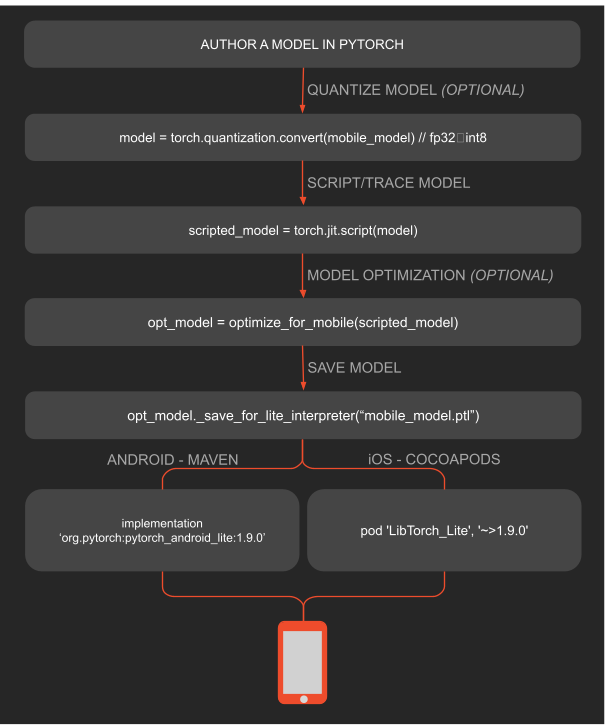
\includegraphics[width=0.5\textwidth]{Immagini/workflow_pytorch.png}
    \caption{Workflow dal training al rilascio di un modello su piattaforma mobile.}
    \label{fig:pyworkflow}
\end{figure}

\subsection{Quantizzazione}
La quantizzazione\cite{Quantizzazione} è una tecnica utilizzata principalmente per accelerare la fase di inferenza nei modelli di machine learning,
rendendo più veloce l'elaborazione delle previsioni o delle decisioni basate sui dati. Questo metodo funziona riducendo la precisione dei numeri utilizzati;
questo serve per avere una rappresentazione del modello più compatta e per poter utilizzare operazioni vettoriali più efficientemente su molti hardware.
Partendo da un modello FP32 (Floating Point 32 bit), PyTorch supporta la quantizzazione INT8 (Integer 8 bit), ottenendo così una riduzione della dimensione
del modello e della necessità di memoria di 4 volte. Inoltre il supporto hardware per la computazione INT8 è solitamente 2 o addirittura 4 volte più veloce
rispetto a quella FP32. Queste tecniche si utilizzano principalmente nella fase di inferenza del modello ("only the forward pass is supported for quantized operators"),
e non durante la fase di addestramento.

PyTorch fornisce tre differenti modalità per la quantizzazione:
\begin{itemize}
    \item Eager Mode Quantization (beta)
    \item FX Graph Mode Quantization (prototipo)
    \item PyTorch 2 Export Quantization
\end{itemize}
\subsubsection{Eager Mode Quantization}
Questa funzionalità, ancora in versione beta, richiede che l'utente gestisca manualmente le fasi di quantizzazione e dequantizzazione.
Supporta solamente i moduli\footnote{In PyTorch, un modulo (classe torch.nn.Module) rappresenta un componente di un modello che incapsula uno o più strati, parametri e una funzione di forward che definisce come l'input viene trasformato in output. Possono avere uno stato, ossia dei pesi aggiornati durante il training,}
e non le funzioni\footnote{Spesso presenti nel modulo torch.nn.functional, sono operazioni stateless che eseguono calcoli specifici come attivazioni (ReLU, sigmoid), operazioni di pooling, e altre trasformazioni matematiche. Non mantengono uno stato.}.

\subsubsection{FX Graph Mode Quantization}
Al contrario del primo, questo modo di effettuare la quantizzazione è automatizzato. Migliora la Eager Mode aggiungendo il supporto per le funzioni,
anche se potrebbe essere necessario effettuare un refactor del modello per renderlo compatibile con la modalità FX.

\subsubsection{PyTorch 2 Export Quantization}
Questa è la nuova modalità di quantizzazione completa del grafo, e può essere utilizzata da una percentuale più elevata di modelli rispetto alla
modalità grafica FX, anche se presenta ancora limitazioni riguardo alcuni costrutti Python e richiede l'intervento dell'utente per supportare il
dinamismo nel modello esportato. Le caratteristiche principali sono:
\begin{enumerate}
    \item API programmabili per configurare come un modello viene quantizzato.
    \item UX (User Experience) semplificata per gli utenti e per gli sviluppatori backend, poiché è necessario interagire con un singolo oggetto, chiamato \textit{Quantizer}.
    \item Rappresentazione (opzionale) del modello quantizzato di riferimento che può rappresentare calcoli quantizzati con operazioni intere più vicine agli attuali calcoli quantizzati che avvengono nell'hardware.
\end{enumerate}

Ci sono poi tre tipi di quantizzazione supportati, è inoltre possibile vedere quali operatori sono compatibili con i tipi di quantizzazione in figura \ref{fig:quantizationCoverage}:
\begin{itemize}
    \item Quantizzazione dinamica: pesi quantizzati con \textit{activations}\footnote{Le attivazioni, nel contesto del machine learning,
    si riferiscono ai valori di output prodotti dai neuroni di una rete neurale durante il processo di forward pass, ovvero quando l'input viene
    elaborato attraverso i vari strati della rete fino a generare un output.} lette/salvate in floating point e quantizzate per i calcoli;
    \item Quantizzazione statica: pesi e activations quantizzati, è necessaria una fase di calibrazione per determinare i migliori parametri di quantizzazione dopo l'addestramento;
    \item Quantizzazione statica \textit{aware training}: pesi e activations quantizzati, i parametri sono modellati durante l'allenamento.
\end{itemize}

\begin{figure}[ht]
    \centering
    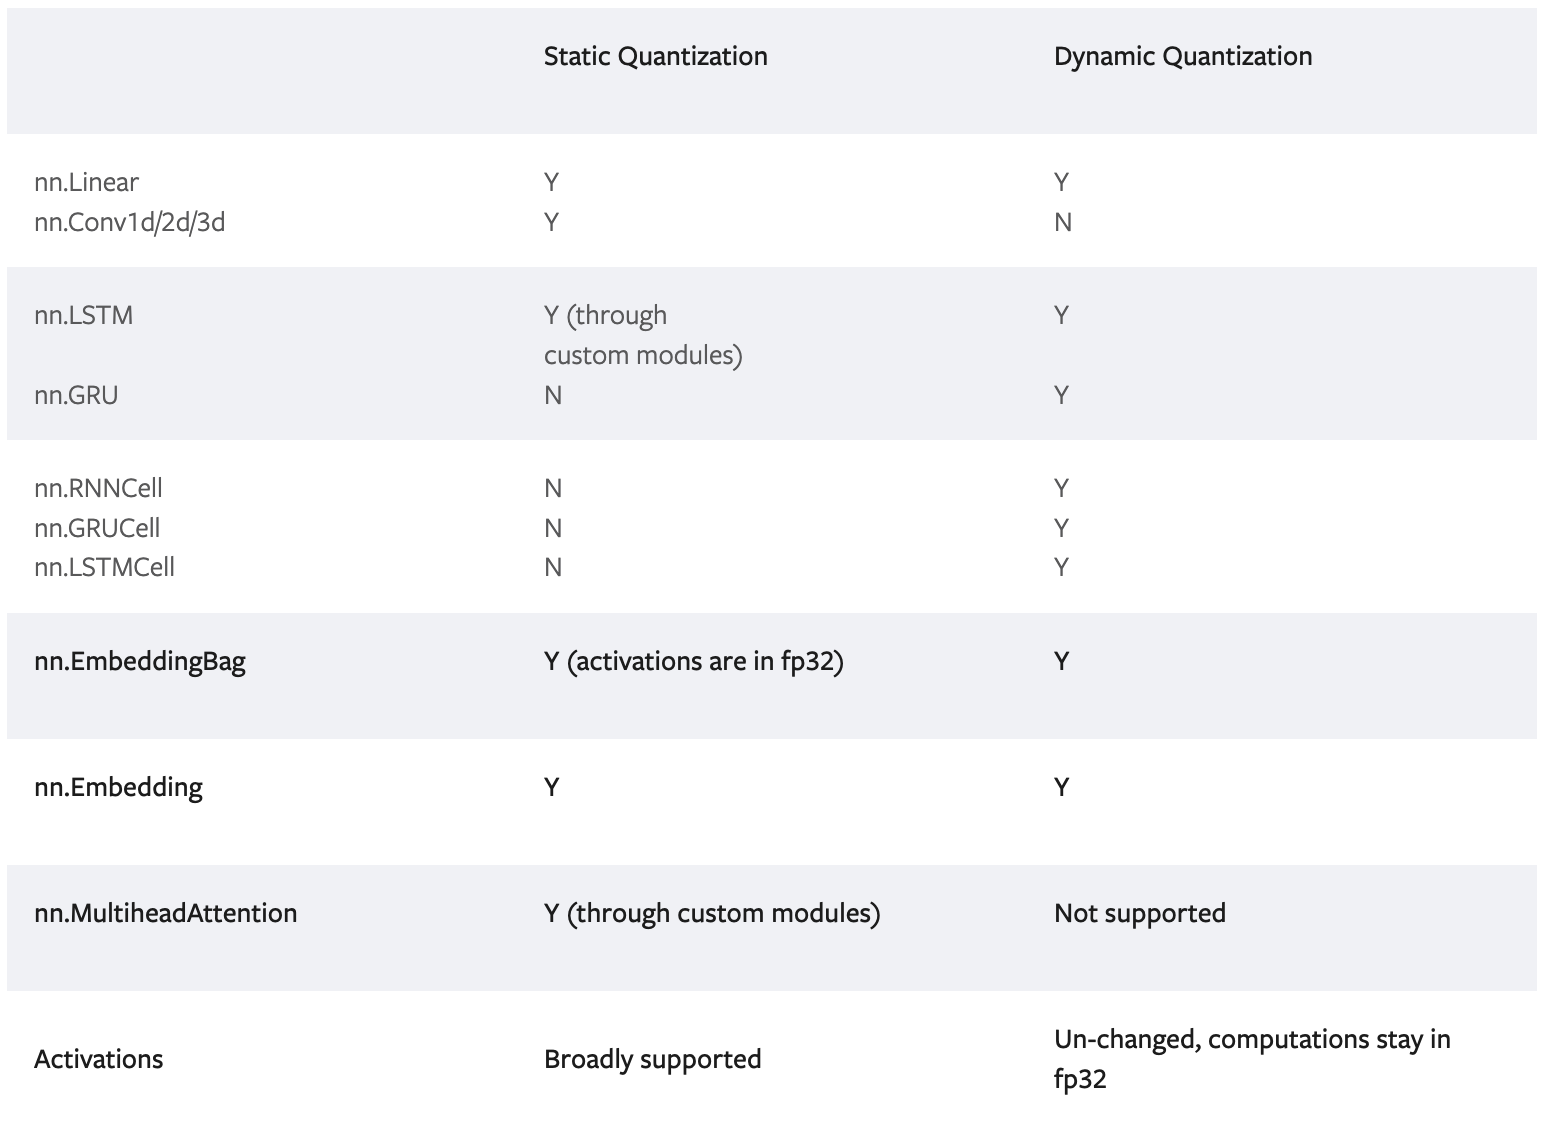
\includegraphics[width=0.8\textwidth]{Immagini/operator coverage.png}
    \caption{Operatori compatibili con i due diversi tipi di quantizzazione}
    \label{fig:quantizationCoverage}
\end{figure}
    
\subsection{Scripting e Tracing del modello}
Questi due step\cite{TracingVSScripting} servono per convertire un \textit{nn.Module} in un grafo in formato TorchScript.
\begin{itemize}
    \item \textbf{Tracing} usa il comando \texttt{torch.jit.trace()}, in cui si passano come argomenti il modello e un input d'esempio. L'input verrà processato
    dal modello e le operazioni eseguite verranno appunto tracciate e registrate in un grafo.
    \item \textbf{Scripting} usa il comando \texttt{torch.jit.script()} che prende in input il solo il modello, in questo caso il modello verrà ispezionato
    staticamente e da questa analisi verrà generato il codice TorchScript.
\end{itemize}
Viene usato prevalentemente il metodo Scripting, poiché cattura sia le operazioni che tutta la logica del modello, inoltre se l'esportazione dovesse fallire sarà
quasi sicuramente per una ragione ben definita (di conseguenza la modifica da apportare sarà chiara). Il Tracing viene preferito quando non si ha accesso al codice
e quindi non è possibile apportare modifiche. È possibile anche utilizzarli insieme.

\subsection{Ottimizzazione}
\label{sec:ottimizzazione}
Grazie alla funzionalità \texttt{torch.utils.mobile\_optimizer.optimize\_for\_mobile}\cite{Ottimizzazione} si semplifica il processo di ottimizzazione
di modelli per garantire che funzionino in modo efficiente su piattaforme con risorse limitate, come gli smartphone e i tablet.
Il comando \texttt{torch.utils.mobile\_optimizer.optimize\_for\_mobile(script\_module, optimization\_blocklist=None, preserved\_methods=None, backend='CPU')} esegue
diverse operazioni in base ai parametri passati:
\begin{enumerate}
    \item \textit{script\_module}: un'istanza del modello TorchScript;
    \item \textit{optimization\_blocklist}: ottimizzazioni da escludere tra quelle disponibili;
    \item \textit{preserved\_methods}: lista di metodi che devono essere mantenuti quando si invoca \texttt{freeze\_module};
    \item \textit{backend}: tipo di dispositivo usato per eseguire il modello risultante (CPU di default, oppure "Vulkan" o "Metal").
\end{enumerate}

In caso non si passi una lista di ottimizzazioni da non eseguire, vengono eseguite tutte le seguenti:
\begin{itemize}
    \item Conv2D + BatchNorm fusion: combina operazioni Conv2d\footnote{Applica una convoluzione 2D su un segnale di ingresso composto da diversi piani di ingresso.}
    e BatchNorm2d\footnote{Applica la Batch Normalization ad un input 4D.} in un'unica operazione Conv2d, aggiornando i relativi pesi e bias.
    \item Insert and Fold prepacked ops: sostituisce le operazioni Conv2D e le operazioni lineari con le loro controparti preconfezionate, ottimizzando l'accesso alla memoria e l'esecuzione del kernel.
    \item ReLU/Hardtanh fusion: integra operazioni di ReLU\footnote{Applica la funzione rectified linear unit elemento per elemento} o
    Hardtanh\footnote{Applica la funzione HardTanh function elemento per elemento} con le operazioni Conv2D o lineari precedenti, sfruttando l'ottimizzazione hardware XNNPACK.
    \item Dropout removal: elimina i nodi di dropout\footnote{Durante l'addestramento, azzera casualmente alcuni elementi del tensore di input
    con probabilità p} dal modello quando il training è impostato su false.
    \item Conv packed params hoisting:sposta i parametri impacchettati delle convoluzioni al modulo radice, riducendo la dimensione del modello senza
    influire sui risultati numerici.
    \item Add/ReLU fusion: trova e combina operazioni di addizione seguite da ReLU in un'unica operazione \texttt{add\_relu}.
\end{itemize}

